%% bare_jrnl.tex
%% V1.4b
%% 2015/08/26
%% by Michael Shell
%% see http://www.michaelshell.org/
%% for current contact information.
%%
%% This is a skeleton file demonstrating the use of IEEEtran.cls
%% (requires IEEEtran.cls version 1.8b or later) with an IEEE
%% journal paper.
%%
%% Support sites:
%% http://www.michaelshell.org/tex/ieeetran/
%% http://www.ctan.org/pkg/ieeetran
%% and
%% http://www.ieee.org/


%%*************************************************************************
%% Legal Notice:
%% This code is offered as-is without any warranty either expressed or
%% implied; without even the implied warranty of MERCHANTABILITY or
%% FITNESS FOR A PARTICULAR PURPOSE! 
%% User assumes all risk.
%% In no event shall the IEEE or any contributor to this code be liable for
%% any damages or losses, including, but not limited to, incidental,
%% consequential, or any other damages, resulting from the use or misuse
%% of any information contained here.
%%
%% All comments are the opinions of their respective authors and are not
%% necessarily endorsed by the IEEE.
%%
%% This work is distributed under the LaTeX Project Public License (LPPL)
%% ( http://www.latex-project.org/ ) version 1.3, and may be freely used,
%% distributed and modified. A copy of the LPPL, version 1.3, is included
%% in the base LaTeX documentation of all distributions of LaTeX released
%% 2003/12/01 or later.
%% Retain all contribution notices and credits.
%% ** Modified files should be clearly indicated as such, including  **
%% ** renaming them and changing author support contact information. **
%%*************************************************************************


% *** Authors should verify (and, if needed, correct) their LaTeX system  ***
% *** with the testflow diagnostic prior to trusting their LaTeX platform ***
% *** with production work. The IEEE's font choices and paper sizes can   ***
% *** trigger bugs that do not appear when using other class files.       ***                          ***
% The testflow support page is at:
% http://www.michaelshell.org/tex/testflow/

%
\documentclass[conference]{./pvsctran}
%
% If IEEEtran.cls has not been installed into the LaTeX system files,
% manually specify the path to it like:
% \documentclass[journal]{../sty/IEEEtran}

%\input epsf
\usepackage{graphicx}
\usepackage{hyperref}
\usepackage{graphicx}
\usepackage{amssymb}
\usepackage{amsmath}
\usepackage[super]{nth}
\usepackage{multicol}



% Some very useful LaTeX packages include:
% (uncomment the ones you want to load)


% *** MISC UTILITY PACKAGES ***
%
%\usepackage{ifpdf}
% Heiko Oberdiek's ifpdf.sty is very useful if you need conditional
% compilation based on whether the output is pdf or dvi.
% usage:
% \ifpdf
%   % pdf code
% \else
%   % dvi code
% \fi
% The latest version of ifpdf.sty can be obtained from:
% http://www.ctan.org/pkg/ifpdf
% Also, note that IEEEtran.cls V1.7 and later provides a builtin
% \ifCLASSINFOpdf conditional that works the same way.
% When switching from latex to pdflatex and vice-versa, the compiler may
% have to be run twice to clear warning/error messages.






% *** CITATION PACKAGES ***
%
%\usepackage{cite}
% cite.sty was written by Donald Arseneau
% V1.6 and later of IEEEtran pre-defines the format of the cite.sty package
% \cite{} output to follow that of the IEEE. Loading the cite package will
% result in citation numbers being automatically sorted and properly
% "compressed/ranged". e.g., [1], [9], [2], [7], [5], [6] without using
% cite.sty will become [1], [2], [5]--[7], [9] using cite.sty. cite.sty's
% \cite will automatically add leading space, if needed. Use cite.sty's
% noadjust option (cite.sty V3.8 and later) if you want to turn this off
% such as if a citation ever needs to be enclosed in parenthesis.
% cite.sty is already installed on most LaTeX systems. Be sure and use
% version 5.0 (2009-03-20) and later if using hyperref.sty.
% The latest version can be obtained at:
% http://www.ctan.org/pkg/cite
% The documentation is contained in the cite.sty file itself.






% *** GRAPHICS RELATED PACKAGES ***
%
\ifCLASSINFOpdf
  % \usepackage[pdftex]{graphicx}
  % declare the path(s) where your graphic files are
  % \graphicspath{{../pdf/}{../jpeg/}}
  % and their extensions so you won't have to specify these with
  % every instance of \includegraphics
  % \DeclareGraphicsExtensions{.pdf,.jpeg,.png}
\else
  % or other class option (dvipsone, dvipdf, if not using dvips). graphicx
  % will default to the driver specified in the system graphics.cfg if no
  % driver is specified.
  % \usepackage[dvips]{graphicx}
  % declare the path(s) where your graphic files are
  % \graphicspath{{../eps/}}
  % and their extensions so you won't have to specify these with
  % every instance of \includegraphics
  % \DeclareGraphicsExtensions{.eps}
\fi
% graphicx was written by David Carlisle and Sebastian Rahtz. It is
% required if you want graphics, photos, etc. graphicx.sty is already
% installed on most LaTeX systems. The latest version and documentation
% can be obtained at: 
% http://www.ctan.org/pkg/graphicx
% Another good source of documentation is "Using Imported Graphics in
% LaTeX2e" by Keith Reckdahl which can be found at:
% http://www.ctan.org/pkg/epslatex
%
% latex, and pdflatex in dvi mode, support graphics in encapsulated
% postscript (.eps) format. pdflatex in pdf mode supports graphics
% in .pdf, .jpeg, .png and .mps (metapost) formats. Users should ensure
% that all non-photo figures use a vector format (.eps, .pdf, .mps) and
% not a bitmapped formats (.jpeg, .png). The IEEE frowns on bitmapped formats
% which can result in "jaggedy"/blurry rendering of lines and letters as
% well as large increases in file sizes.
%
% You can find documentation about the pdfTeX application at:
% http://www.tug.org/applications/pdftex





% *** MATH PACKAGES ***
%
%\usepackage{amsmath}
% A popular package from the American Mathematical Society that provides
% many useful and powerful commands for dealing with mathematics.
%
% Note that the amsmath package sets \interdisplaylinepenalty to 10000
% thus preventing page breaks from occurring within multiline equations. Use:
%\interdisplaylinepenalty=2500
% after loading amsmath to restore such page breaks as IEEEtran.cls normally
% does. amsmath.sty is already installed on most LaTeX systems. The latest
% version and documentation can be obtained at:
% http://www.ctan.org/pkg/amsmath





% *** SPECIALIZED LIST PACKAGES ***
%
%\usepackage{algorithmic}
% algorithmic.sty was written by Peter Williams and Rogerio Brito.
% This package provides an algorithmic environment fo describing algorithms.
% You can use the algorithmic environment in-text or within a figure
% environment to provide for a floating algorithm. Do NOT use the algorithm
% floating environment provided by algorithm.sty (by the same authors) or
% algorithm2e.sty (by Christophe Fiorio) as the IEEE does not use dedicated
% algorithm float types and packages that provide these will not provide
% correct IEEE style captions. The latest version and documentation of
% algorithmic.sty can be obtained at:
% http://www.ctan.org/pkg/algorithms
% Also of interest may be the (relatively newer and more customizable)
% algorithmicx.sty package by Szasz Janos:
% http://www.ctan.org/pkg/algorithmicx




% *** ALIGNMENT PACKAGES ***
%
%\usepackage{array}
% Frank Mittelbach's and David Carlisle's array.sty patches and improves
% the standard LaTeX2e array and tabular environments to provide better
% appearance and additional user controls. As the default LaTeX2e table
% generation code is lacking to the point of almost being broken with
% respect to the quality of the end results, all users are strongly
% advised to use an enhanced (at the very least that provided by array.sty)
% set of table tools. array.sty is already installed on most systems. The
% latest version and documentation can be obtained at:
% http://www.ctan.org/pkg/array


% IEEEtran contains the IEEEeqnarray family of commands that can be used to
% generate multiline equations as well as matrices, tables, etc., of high
% quality.




% *** SUBFIGURE PACKAGES ***
%\ifCLASSOPTIONcompsoc
%  \usepackage[caption=false,font=normalsize,labelfont=sf,textfont=sf]{subfig}
%\else
%  \usepackage[caption=false,font=footnotesize]{subfig}
%\fi
% subfig.sty, written by Steven Douglas Cochran, is the modern replacement
% for subfigure.sty, the latter of which is no longer maintained and is
% incompatible with some LaTeX packages including fixltx2e. However,
% subfig.sty requires and automatically loads Axel Sommerfeldt's caption.sty
% which will override IEEEtran.cls' handling of captions and this will result
% in non-IEEE style figure/table captions. To prevent this problem, be sure
% and invoke subfig.sty's "caption=false" package option (available since
% subfig.sty version 1.3, 2005/06/28) as this is will preserve IEEEtran.cls
% handling of captions.
% Note that the Computer Society format requires a larger sans serif font
% than the serif footnote size font used in traditional IEEE formatting
% and thus the need to invoke different subfig.sty package options depending
% on whether compsoc mode has been enabled.
%
% The latest version and documentation of subfig.sty can be obtained at:
% http://www.ctan.org/pkg/subfig




% *** FLOAT PACKAGES ***
%
%\usepackage{fixltx2e}
% fixltx2e, the successor to the earlier fix2col.sty, was written by
% Frank Mittelbach and David Carlisle. This package corrects a few problems
% in the LaTeX2e kernel, the most notable of which is that in current
% LaTeX2e releases, the ordering of single and double column floats is not
% guaranteed to be preserved. Thus, an unpatched LaTeX2e can allow a
% single column figure to be placed prior to an earlier double column
% figure.
% Be aware that LaTeX2e kernels dated 2015 and later have fixltx2e.sty's
% corrections already built into the system in which case a warning will
% be issued if an attempt is made to load fixltx2e.sty as it is no longer
% needed.
% The latest version and documentation can be found at:
% http://www.ctan.org/pkg/fixltx2e


%\usepackage{stfloats}
% stfloats.sty was written by Sigitas Tolusis. This package gives LaTeX2e
% the ability to do double column floats at the bottom of the page as well
% as the top. (e.g., "\begin{figure*}[!b]" is not normally possible in
% LaTeX2e). It also provides a command:
%\fnbelowfloat
% to enable the placement of footnotes below bottom floats (the standard
% LaTeX2e kernel puts them above bottom floats). This is an invasive package
% which rewrites many portions of the LaTeX2e float routines. It may not work
% with other packages that modify the LaTeX2e float routines. The latest
% version and documentation can be obtained at:
% http://www.ctan.org/pkg/stfloats
% Do not use the stfloats baselinefloat ability as the IEEE does not allow
% \baselineskip to stretch. Authors submitting work to the IEEE should note
% that the IEEE rarely uses double column equations and that authors should try
% to avoid such use. Do not be tempted to use the cuted.sty or midfloat.sty
% packages (also by Sigitas Tolusis) as the IEEE does not format its papers in
% such ways.
% Do not attempt to use stfloats with fixltx2e as they are incompatible.
% Instead, use Morten Hogholm'a dblfloatfix which combines the features
% of both fixltx2e and stfloats:
%
% \usepackage{dblfloatfix}
% The latest version can be found at:
% http://www.ctan.org/pkg/dblfloatfix




%\ifCLASSOPTIONcaptionsoff
%  \usepackage[nomarkers]{endfloat}
% \let\MYoriglatexcaption\caption
% \renewcommand{\caption}[2][\relax]{\MYoriglatexcaption[#2]{#2}}
%\fi
% endfloat.sty was written by James Darrell McCauley, Jeff Goldberg and 
% Axel Sommerfeldt. This package may be useful when used in conjunction with 
% IEEEtran.cls'  captionsoff option. Some IEEE journals/societies require that
% submissions have lists of figures/tables at the end of the paper and that
% figures/tables without any captions are placed on a page by themselves at
% the end of the document. If needed, the draftcls IEEEtran class option or
% \CLASSINPUTbaselinestretch interface can be used to increase the line
% spacing as well. Be sure and use the nomarkers option of endfloat to
% prevent endfloat from "marking" where the figures would have been placed
% in the text. The two hack lines of code above are a slight modification of
% that suggested by in the endfloat docs (section 8.4.1) to ensure that
% the full captions always appear in the list of figures/tables - even if
% the user used the short optional argument of \caption[]{}.
% IEEE papers do not typically make use of \caption[]'s optional argument,
% so this should not be an issue. A similar trick can be used to disable
% captions of packages such as subfig.sty that lack options to turn off
% the subcaptions:
% For subfig.sty:
% \let\MYorigsubfloat\subfloat
% \renewcommand{\subfloat}[2][\relax]{\MYorigsubfloat[]{#2}}
% However, the above trick will not work if both optional arguments of
% the \subfloat command are used. Furthermore, there needs to be a
% description of each subfigure *somewhere* and endfloat does not add
% subfigure captions to its list of figures. Thus, the best approach is to
% avoid the use of subfigure captions (many IEEE journals avoid them anyway)
% and instead reference/explain all the subfigures within the main caption.
% The latest version of endfloat.sty and its documentation can obtained at:
% http://www.ctan.org/pkg/endfloat
%
% The IEEEtran \ifCLASSOPTIONcaptionsoff conditional can also be used
% later in the document, say, to conditionally put the References on a 
% page by themselves.




% *** PDF, URL AND HYPERLINK PACKAGES ***
%
%\usepackage{url}
% url.sty was written by Donald Arseneau. It provides better support for
% handling and breaking URLs. url.sty is already installed on most LaTeX
% systems. The latest version and documentation can be obtained at:
% http://www.ctan.org/pkg/url
% Basically, \url{my_url_here}.




% *** Do not adjust lengths that control margins, column widths, etc. ***
% *** Do not use packages that alter fonts (such as pslatex).         ***
% There should be no need to do such things with IEEEtran.cls V1.6 and later.
% (Unless specifically asked to do so by the journal or conference you plan
% to submit to, of course. )


% correct bad hyphenation here
\hyphenation{op-tical net-works semi-conduc-tor}


\begin{document}
%
% paper title
% Titles are generally capitalized except for words such as a, an, and, as,
% at, but, by, for, in, nor, of, on, or, the, to and up, which are usually
% not capitalized unless they are the first or last word of the title.
% Linebreaks \\ can be used within to get better formatting as desired.
% Do not put math or special symbols in the title.
\title{\LARGE Manuscript Preparation Guidelines and Template for the 46th IEEE Photovoltaic Specialists Conference (Title in 18-point Times font)}


% author names and affiliations
% use a multiple column layout for up to three different
% affiliations
\author{ \IEEEauthorblockN{\large William Shockley, Hans Queisser, and William R. Cherry   (List authors on this line using 12 point Times \\font -- use a second line if necessary)} \\
\IEEEauthorblockA{\large Institute Name, City, State/Region, Mail/Zip Code, Country (authors' affiliation(s) listed here in 12 point\\ Times font Ð use a second line if necessary)}}

% conference papers do not typically use \thanks and this command
% is locked out in conference mode. If really needed, such as for
% the acknowledgment of grants, issue a \IEEEoverridecommandlockouts
% after \documentclass

% for over three affiliations, or if they all won't fit within the width
% of the page, use this alternative format:
% 
%\author{\IEEEauthorblockN{Michael Shell\IEEEauthorrefmark{1},
%Homer Simpson\IEEEauthorrefmark{2},
%James Kirk\IEEEauthorrefmark{3}, 
%Montgomery Scott\IEEEauthorrefmark{3} and
%Eldon Tyrell\IEEEauthorrefmark{4}}
%\IEEEauthorblockA{\IEEEauthorrefmark{1}School of Electrical and Computer Engineering\\
%Georgia Institute of Technology,
%Atlanta, Georgia 30332--0250\\ Email: see http://www.michaelshell.org/contact.html}
%\IEEEauthorblockA{\IEEEauthorrefmark{2}Twentieth Century Fox, Springfield, USA\\
%Email: homer@thesimpsons.com}
%\IEEEauthorblockA{\IEEEauthorrefmark{3}Starfleet Academy, San Francisco, California 96678-2391\\
%Telephone: (800) 555--1212, Fax: (888) 555--1212}
%\IEEEauthorblockA{\IEEEauthorrefmark{4}Tyrell Inc., 123 Replicant Street, Los Angeles, California 90210--4321}}




% use for special paper notices
%\IEEEspecialpapernotice{(Invited Paper)}

\setlength{\columnsep}{0.25in}


% make the title area
\maketitle


\begin{abstract}
%\boldmath
An abstract in the two-column format is required for the manuscript. Use 9 point Times New Roman Bold font for the abstract. Set your line spacing to be 10 points rather than single space. Indent the first line by 0.125 inches and type the word ``Abstract'' in 9 point Times New Roman Bold Italic. This should be followed by two spaces, a long dash (option / shift / minus), two spaces, and then the first word of your abstract (as shown above). Please try to keep the length of your abstract to 100 words or less. Times font is an acceptable substitute for Times New Roman font. After the abstract, you should list a few key words that describe your paper. Typically, you should list about 5 to 7 key words, in alphabetical order, using 9 point Times New Roman Bold font.
\end{abstract}
% IEEEtran.cls defaults to using nonbold math in the Abstract.
% This preserves the distinction between vectors and scalars. However,
% if the conference you are submitting to favors bold math in the abstract,
% then you can use LaTeX's standard command \boldmath at the very start
% of the abstract to achieve this. Many IEEE journals/conferences frown on
% math in the abstract anyway.
\begin{IEEEkeywords}
amorphous materials, charge carrier lifetime, photovoltaic cells, silicon.
\end{IEEEkeywords}
% no keywords




% For peer review papers, you can put extra information on the cover
% page as needed:
% \ifCLASSOPTIONpeerreview
% \begin{center} \bfseries EDICS Category: 3-BBND \end{center}
% \fi
%
% For peerreview papers, this IEEEtran command inserts a page break and
% creates the second title. It will be ignored for other modes.
\IEEEpeerreviewmaketitle



\section{Introduction}
Please follow these instructions carefully.  Papers not meeting these guidelines may be excluded from the conference proceedings.  These instructions have been formatted in the manner in which you should prepare your manuscript; you may use this TeX document as a template.  Please use this as an example.  For details or clarification, please contact the Publications Chair at \url{Publications@ieee-pvsc.org}. 

Please read through this entire template before you start using it to create your paper! This will save you and the PVSC considerable time. A contributor should remember that:
\hfil\break
1) Deadline to submit this paper is \textbf{June 3, 2019!}\\
2) Manuscripts must be submitted electronically to the conference website (\url{http://www.ieee-pvsc.org}).  Manuscripts must be submitted in either Microsoft Word or PDF format.  No hardcopy is required.  If you submit a Microsoft Word document, it will be converted to PDF format.  Be sure to doownload and view this PDF document to ensure proper conversion.  \\
3) If the manuscript is not submitted by the \textbf{June 3, 2019!}\\ deadline, presentation and publication will not be permitted.  In addition, no manuscript will be published without presentation at the conference.  PVSC FOLLOWS A STRICT NO PAPER-NO PODIUM AND NO PODIUM-NO PAPER RULE.  Should you have any difficulty with the electronic submission process, please contact SPLTrak at \url{help@SPLTrak.com}.\\ 
4) All papers are limited to six (8) pages (including all figures) and 2 MB file size.\\
5)	You should employ this format. This document is being made available as a template for your convenience. If you elect not to use this template, please remember that you must still adhere to the general guidelines embodied in this document concerning, but not limited to, font size, margin size, page limits, file size, etc.\\
\begin{table*}
\centerline { TABLE 1  } 
\vskip5pt
\centerline { \normalsize \textsc{Summary of Typographical Settings}}
\vskip2pt
\centerline{
\vbox{\offinterlineskip
\hrule
%\vskip2pt\hrule\vskip2pt
% Leading & means preamble template repeats infinitely. p.241 TeX Book.
\halign{&\vrule#&
\strut\quad#\hfil\quad\cr
%Use either first and third lines following this description, OR the
%second line.  The first choice is used when all vertical rules go to the
%top of the first horizontal line of the table.  The second choice below
%(with the \strut) is used when there are column headings that span
%more than one column.  The \strut in that column line will not have the
%vertical tic marks in the horizontal rule.  Note that a vrule is also
%considered a column, so when using \multispanx, x is the number of
%all columns including the ``vrule.'' 
%height2pt&\omit&&\omit&&\omit&&\omit&&\omit&&\omit&&\omit&&\omit&&\omit&\cr
&\strut &&\multispan5\hfil {\bf Font Specifics}\hfil&&\multispan9\hfil {\bf Paragraph Description}\hfil &\cr
%&\omit &&\multispan5\hfil {\bf Font Specifics}\hfil&&\multispan9\hfil {\bf Paragraph Description}\hfil &\cr
&{\bf Section}&&\multispan5\hfil (Times Roman unless
specified)\hfil&&\multispan5\hfil spacing (in points)\hfil &&
alignment&&indent&\cr
&\omit&&style&&size&&special&&line&&before&&after&&\omit&&(in inches)&\cr
height2pt&\omit&&\omit&&\omit&&\omit&&\omit&&\omit&&\omit&&\omit&&\omit&\cr
\noalign{\hrule}
height2pt&\omit&&\omit&&\omit&&\omit&&\omit&&\omit&&\omit&&\omit&&\omit&\cr
%\noalign{\vskip2pt\hrule\vskip2pt}
%\omit&\omit&\omit&\omit\cr
&Title&&plain&&18&&none&&single&&6&&6&&centered&&none&\cr
&Autohr List&&plain&&12&&none&&single&&6&&6&&centered&&none&\cr
&Affiliations&&plain&&12&&none&&single&&6&&6&&centered&&none&\cr
&Abstract&&bold&&9&&none&&exactly 10&&0&&0&&justified&&0.125 $1^{st}$ line&\cr
&Headings&&plain&&10&&small caps&&exactly 12&&18&&6&&centered&&none&\cr
&Subheadings&&italic&&10&&none&&exactly 12&&6&&6&&left&&none&\cr
&Body Paragraphs&&plain&&10&&none&&exactly 12&&0&&0&&justified&&0.125 $1^{st}$ line&\cr
&Equations&&\multispan5 \hfil Symbol font for special characters
\hfil&&single&&6&&6&&centered&&none&\cr
&Figures&&\multispan5 \hfil 8 to 10 point sans serif (Helvetica)\hfil&&single&&0&&0&&centered&&none&\cr
&Figure Captions&&plain&&9&&none &&10&&0&&0&&justified&&none, tab at 0.5&\cr
&References&&plain&&9&&none&&10&&0&&0&&justified&&0.25 hanging&\cr
height2pt&\omit&&\omit&&\omit&&\omit&&\omit&&\omit&&\omit&&\omit&&\omit&\cr}
\hrule}}
\label{table1}
\end{table*}

\section{Detailed Text Formatting}
Use a two column format.  All paragraphs of text, including the abstract, figure captions, and references, should be justified at the left and the right edges.

Please do not include page numbers, headers or footers.  Company logos should not be inserted into a header or footer.  \textbf{YOUR MANUSCRIPT WILL BE REJECTED IF THERE ARE PAGE NUMBERS, HEADERS OR FOOTERS.}  This is to allow IEEE to add their official footer information and allow for IEEE to determine page numbering if appropriate.

For the Title, use 18-point Times (Roman) font. Its paragraph description should be set so that the line spacing is single with 6-point spacing before and 6-point spacing after. The font description for the Author List and Authors' Affiliation(s) should be 12-point Times. The paragraph descriptions should be set so that the line spacing is single with 6-point spacings before and after. Use an additional line spacing of 12 points before the beginning of the double column section, as shown above.

Using 8.5 x 11-inch paper, the top margin is 0.75 inch, the bottom margin is 1 inch, and the left and right margins are
0.625 inch. Except for Title, Authors and Affiliations, use a double column format. The column width is 3.5 inches and the column spacing is 0.25 inch.

Each major section begins with a Heading in 10 point Times font centered within the column and numbered using Roman numerals (except for \textsc{Acknowledgment} and \textsc{References}), followed by a period, a single space, and the title using an initial capital letter for each word. The remaining letters are in \textsc{Small Capitals}. The paragraph description of the section heading line should be set for 18 points before, 6 points after, and the line spacing should be set to exactly 12 points.

For the body of your paper, use 10-point Times font and set your line spacing at ``exactly 12 points'' with 0 points before and after. Indent each paragraph by 0.125 inches. 

Further details are provided in the remainder of this paper for specific situations.

\subsection{ Major Subsections}
As shown, denote subsections with left justified 10-point Times Italic. Order them with capitalized alphabetic characters $(A, B,...)$. Follow the letter designation with a period, a single space, and then the subsection title capitalizing the first letter of each word. The paragraph description of the subsection heading is set to "exactly 12-point" line spacing with 6 points before and after.
\subsection{ Equations }
Equations should be centered in the column and numbered sequentially. Place the equation number to the right of the equation within a parenthesis, with right justification within its column. An example would be
\begin{equation}
V_{OC}=\frac{1}{\beta}ln\left(\frac{I_L}{I_S}+1\right)
\end{equation}
\emph{Make sure that any subscripts in your equations are legible and are not too
small to read!} When referring to an equation, use the number within
parenthesis. For example, you would usually refer to the first
equation as (1) rather than equation (1). If possible, use the Symbol
font for all special characters.%, or better yet, use Equation Editor or
%MathType. 
The paragraph description of the line containing the
equation should be set for 6 points before and 6 points after. The
paragraph spacing will need to be set to ``single'' rather than ``exactly
12 point'' so that the height will autoscale to fit the equation.

\section{Figures and Tables}
The use of color in figures and photos is recommended.  Keep in mind that the proceedings will only be produced in electronic format (DVD).  There will not be a hardbound version of the proceedings.  Please consider the use of different line styles (dashes, dots, etc.) in plots to ensure clarity.  See example.  Please use jpg or png format for all images and compress the size.

Most of the following applies to Microsoft Word.  Figures should utilize as much of the column width as possible in order to maximize legibility. Use a sans serif font, such as Helvetica. Helvetica is larger and much easier to read than Times. Using 8- to 10-point Helvetica usually results in a legible figure. \emph{Do not use any font smaller than 8-point!} It must be legible. When referring to a figure, use the abbreviation Fig. followed by its number. Place figure captions directly below each figure. Use
9-point Times with the paragraph spacing set at ``exactly 10 points.'' Set a tab at 0.5 inch. Type ``Fig. \#.'' (\# is the numeral) then tab over to the 0.5 inch mark before beginning the text of the figure caption. Note that figure captions are always (left and right) justified, rather than centered, even if they are less than a single full line in length. See the caption for Fig. 1.

Within \LaTeX, there is basically only one option for placing figures
within your paper.  Often the easiest way is to insert them into the
top of the next column.
%Within Microsoft Word there are several options for placing figures
%within your paper. Often the easiest is to insert them between
%existing paragraphs allowing the figures to remain in that relative
%position. The paragraph description where the figure is inserted must
%be set to ``single'' spacing rather than ``exactly 12 points'' in
%order to allow the line to autoscale in height to display the entire
%figure. Some disadvantages of this approach are that you don't have
%total flexibility in placing figures, and that the figures will move
%as text is inserted or deleted in any part of the document before the
%figure. If you elect to use this approach, it is recommended that you
%nearly complete the editing of your text before inserting any
%figures. Remember to allow room for them, however. Then begin
%inserting figures starting from the beginning of your document. 
Do not lump all figures at the end of the paper!
If you have difficulties with the titles on your figures, you can always elect to add in the titles as separate text boxes, rather than importing the titles with the graph. This is sometimes helpful in getting a lengthy vertically-oriented title to display correctly.

%\begin{figure}
%%\includegraphics {figure_temp.epsi}
%\epsfxsize=3.25in\epsfbox{figure1.eps}
%\caption{ Estimated relationship between the time an author spends reading these instructions and the quality of the author's digest article.}
%\end{figure}

\begin{figure}
\centering
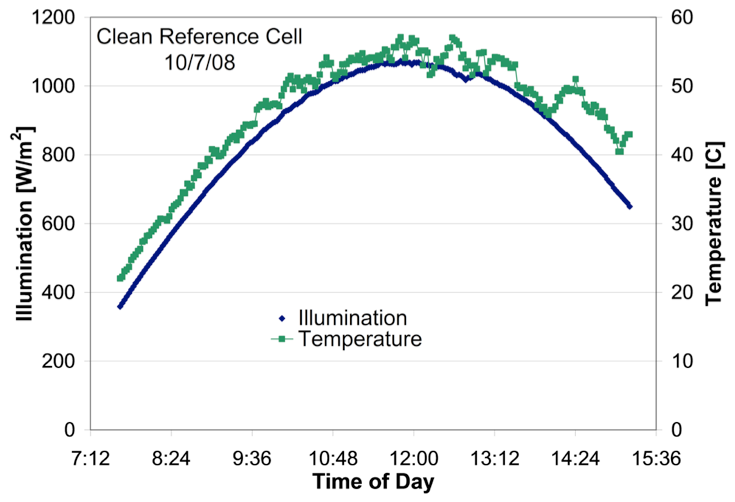
\includegraphics[width=9cm]{image1.png}
\caption{Example of readable plot using different colors and line styles for clarity.}
\end{figure}

Notice that prior to the graph, a single 12-point line is used to
separate the preceding text from the graph. The equivalent of a blank
line should exist between the bottom of the graph (the x-axis caption)
and the figure caption. (In this particular case, there was no need to
add a blank line between the x-axis label and the figure caption,
because there was already adequate spacing provided by the image
border.) After the figure caption, there should be a single 12-point
blank line before the text resumes. 
%\LaTeX accepts encapsulated post script files as figures.  Standard post script figures will not expand and contract to fill the designate area on the page. Encapsulated post script files will.  Thus, encapsulated post script files must obviously be only one page long.  It is often easy to convert a post script file to encapsulated post script.  In Linux this can be done with the command, ``ps2epsi.''
%More flexibility is obtained in inserting figures if you can place
%them exactly where you would like them to be on a page. This can be
%accomplished by inserting the figure, selecting the figure, and then
%choosing ``Format Picture\dots ''. Various settings allow you to place the figure at an absolute position on a page; specify if the text is supposed to flow around the figure or if the figure should move with the text, etc. If you elect to let the text flow around the figure, then remember that you will have to insert a separate text box for the caption, otherwise the figure caption is likely to become separated from the figure.
%When importing a graph from Excel into Word, it is often helpful to
%special-paste it in as a ``Picture (Enhanced Meta-file).'' This saves
%file memory for Word documents. Be aware that the usual Copy
%$\rightarrow $  Paste procedure will copy the entire Excel spreadsheet into your Word file. The Copy $\rightarrow$ Paste Special $\rightarrow$ Picture (Enhanced Metafile) command copies only the graph as a static picture. This is not a concern with PDF file submissions.
If you decide to use color traces in your graphical data, be absolutely certain that there is no ambiguity about your graphical information when printed on a B\&W printer.

Table I on the second page was inserted using ``Insert'', ``Text
Box'', creating the text contained in Table I, and then formatting the
text box using all the settings available under ``Format'', ``Text
Box\dots ''. Table I also serves as an illustration of one of the rare
instances when the double column format requirement can be
violated. Certain figures and tables will require the full-page width
to display. It is usually best to place these figures and tables at
the top, rather than in the middle or bottom of a page. Tables should be entered within a single column if this can be done cleanly, without the entry becoming too crowded.

\section{Citing Previous Work}
When referencing a journal article \cite{Yamaguchi}, a conference
digest article \cite{Hovel} or a book \cite{Fahrenbruch}, place the reference numbers within square
brackets. To simultaneously cite these references \cite{Yamaguchi} - \cite{Fahrenbruch} use the format just demonstrated. The reference list is the last section and references are listed in the order cited. Use 9 point Times. The paragraph description is set for a line spacing of exactly 10 points with 0 point spacing before and after. A 0.25 inch hanging indention should be specified. 

Generally speaking, references should be very detailed. For journal articles, list all authors by initials and last name, the title of the paper in quotations (capitalizing only the first letter of the first word, unless it would be capitalized in a sentence, e.g., a proper noun), the journal name in italics, the volume number, the issue number, the page numbers, and the date. Use the examples provided \cite{Yamaguchi} - \cite{Fahrenbruch} as a guide. 
%Further information on LaTeX and TeX can be found in \cite{IEEEhowto:kopka} - \cite{knuth}. 

% The following statement makes the two columns on the last page more
% or less of equal length.  Placement of this command is by trial and error.
\vfil\eject

\section{Copyright and Reprint Information}
The IEEE copyright form will be electronically submitted for this conference.  On the conference web site, follow the link in the manuscript submission area. 

Reprints may be ordered by checking the appropriate box on the conference registration form.  The reprints will be mailed to you at the address listed on the registration form approximately 3 months after the conference.


\section{Conclusion}
Following these instructions will improve the quality of your paper and the PVSC Proceedings. If you have comments, please contact \url{Publications@ieee-pvsc.org}. Please direct questions regarding the electronic submission process to \url{help@SPLTrak.com}. 

% conference papers do not normally have an appendix

% use section* for acknowledgment



% conference papers do not normally have an appendix


% use section* for acknowledgement



% trigger a \newpage just before the given reference
% number - used to balance the columns on the last page
% adjust value as needed - may need to be readjusted if
% the document is modified later
%\IEEEtriggeratref{8}
% The "triggered" command can be changed if desired:
%\IEEEtriggercmd{\enlargethispage{-5in}}

% references section

% can use a bibliography generated by BibTeX as a .bbl file
% BibTeX documentation can be easily obtained at:
% http://www.ctan.org/tex-archive/biblio/bibtex/contrib/doc/
% The IEEEtran BibTeX style support page is at:
% http://www.michaelshell.org/tex/ieeetran/bibtex/
%\bibliographystyle{IEEEtran}
% argument is your BibTeX string definitions and bibliography database(s)
%\bibliography{IEEEabrv,../bib/paper}
%
% <OR> manually copy in the resultant .bbl file
% set second argument of \begin to the number of references
% (used to reserve space for the reference number labels box)
\begin{thebibliography}{1}
\small

\bibitem {Yamaguchi}
M. Yamaguchi, A. Khan, S.J. Taylor, M. Imaizumi, T. Hisamatsu, and S. Matsuda, ``A detailed model to improve the radiation-resistance of Si space solar cells,\emph{Fundamentals of Solar Cells} vol. 46, pp. 2133-2138, 1999.

\bibitem {Hovel}
H. J. Hovel and J. M. Woodall, ``The effect of depletion region recombination currents on the efficiencies of Si and GaAs solar cells'', \emph {in 10th IEEE Photovoltaic Specialist Conference}, p. 25, 1973.

\bibitem {Fahrenbruch}
A. L. Fahrenbruch and R. H. Bube, \emph{Fundamentals of Solar Cells}, New York: Academic Press, 1983.

%\bibitem{IEEEhowto:kopka}
%H.~Kopka and P.~W. Daly, \emph{A Guide to \LaTeX}, 3rd~ed.\hskip 1em plus
%  0.5em minus 0.4em\relax Harlow, England: Addison-Wesley, 1999.

\end{thebibliography}
%\smallskip
%Note: For the Summary paper submission only, references to the authors own work must be redacted to preserve the new double-blind reviewing requirements.





% that's all folks
\end{document}


